\section{System Call Types}
\label{tach:sec:types}

The C function declarations for syscalls do not describe all
side-effects. \tachyon proposes an extension to the C type
declarations to encode all semantic information necessary to record
which parameters are inputs, which are outputs, and how to identify
all bytes for each parameter. While this problem has been attacked before~\cite{guo:2008},
our particular needs are different due to the binary only-nature of our
approach, as we discuss in \S~\ref{tach:sec:related}.

The \tachyon type system takes advantage of the
user-space/kernel-space barrier for interposition. The barrier
provides a clean separation that can be monitored without
requiring source to the program. In addition, the barrier allows
\tachyon to not monitor internal kernel state. The reason is that the only
way $\unpatched$ and $\patched$ can interact with the underlying
system is via \tachyon, and \tachyon's mechanism ensures that both
programs see an identical state.  This is a vital complexity
reduction.

\tachyon uses a limited form of lightweight dependent types (types
which depend on values). Our lightweight use avoids pitfalls such as
undecidability normally associated with dependent types. In the rest
of this section, we first provide an intuition on the issues and how
dependent types are used, and then describe the full system.


\subsection{Intuition}

A basic approach for recording syscalls is to decorate C types with
information about which parameters should be treated as inputs,
outputs, or both.  We call such annotations the IO class for each
parameter.  In order to specify how to copy output parameters, we also
need to know the size of their values.  The size information is needed
because we need to copy all output bytes from {\tt buf} in the
monitored program $\patched$ to the address space of $\unpatched$.
For example, we could imagine annotating the {\tt read} call as:
\begin{lstlisting}
ssize_t read(int fd, void output* buf{ret}, size_t count);
\end{lstlisting}
The parameter {\tt buf} has been annotated as an output parameter,
thus should be copied and replayed to $\unpatched$.  The annotation
also specifies that {\tt ret} bytes should be copied, where {\tt ret}
is the return value.


Unfortunately, such simple annotations are insufficient with many data
structures, such as vectors. A prime example of a difficult system
call is \texttt{readv}, which provides vectored reads of a file
descriptor. Its C type declaration is:
\begin{lstlisting}
ssize_t readv(int fd, const struct iovec *iov, int iovcnt);
struct iovec {
  void  *iov_base; /* Starting address */
  size_t iov_len; /* Num bytes in iov_base */
};
\end{lstlisting}
The main issue demonstrated is that a complete description of the IO behavior of
parameters may refer to other parameters.  The {\tt iov\_base} length
is determined by {\tt iov\_len}, and the total number of {\tt iov}
items is given by {\tt iovcnt}.  \texttt{readv} is not alone: it has
many friends such as \texttt{writev}, \texttt{preadv}, and
\texttt{pwritev}. In order to handle such cases, we need a type system
that allows us to express \emph{relationships} between parameter values.

% Suddenly, it is less clear exactly how to encode this, and this system
% call is not alone, there are a number of others like it, though it
% and its friends 
% are somewhat unique in that they exercise three cases not addressed by the
% previous system (pointers not in an argument, sizes not in an argument,
% and variable numbers of pointers). In particular, we are now on to a more
% dependent type system, as the exact type is dependent upon a function of the
% values, e.g., the size of the buffer pointed at by \texttt{iov\_base} is
% determined by the lenth next to it.


\begin{figure}
	\begin{center}
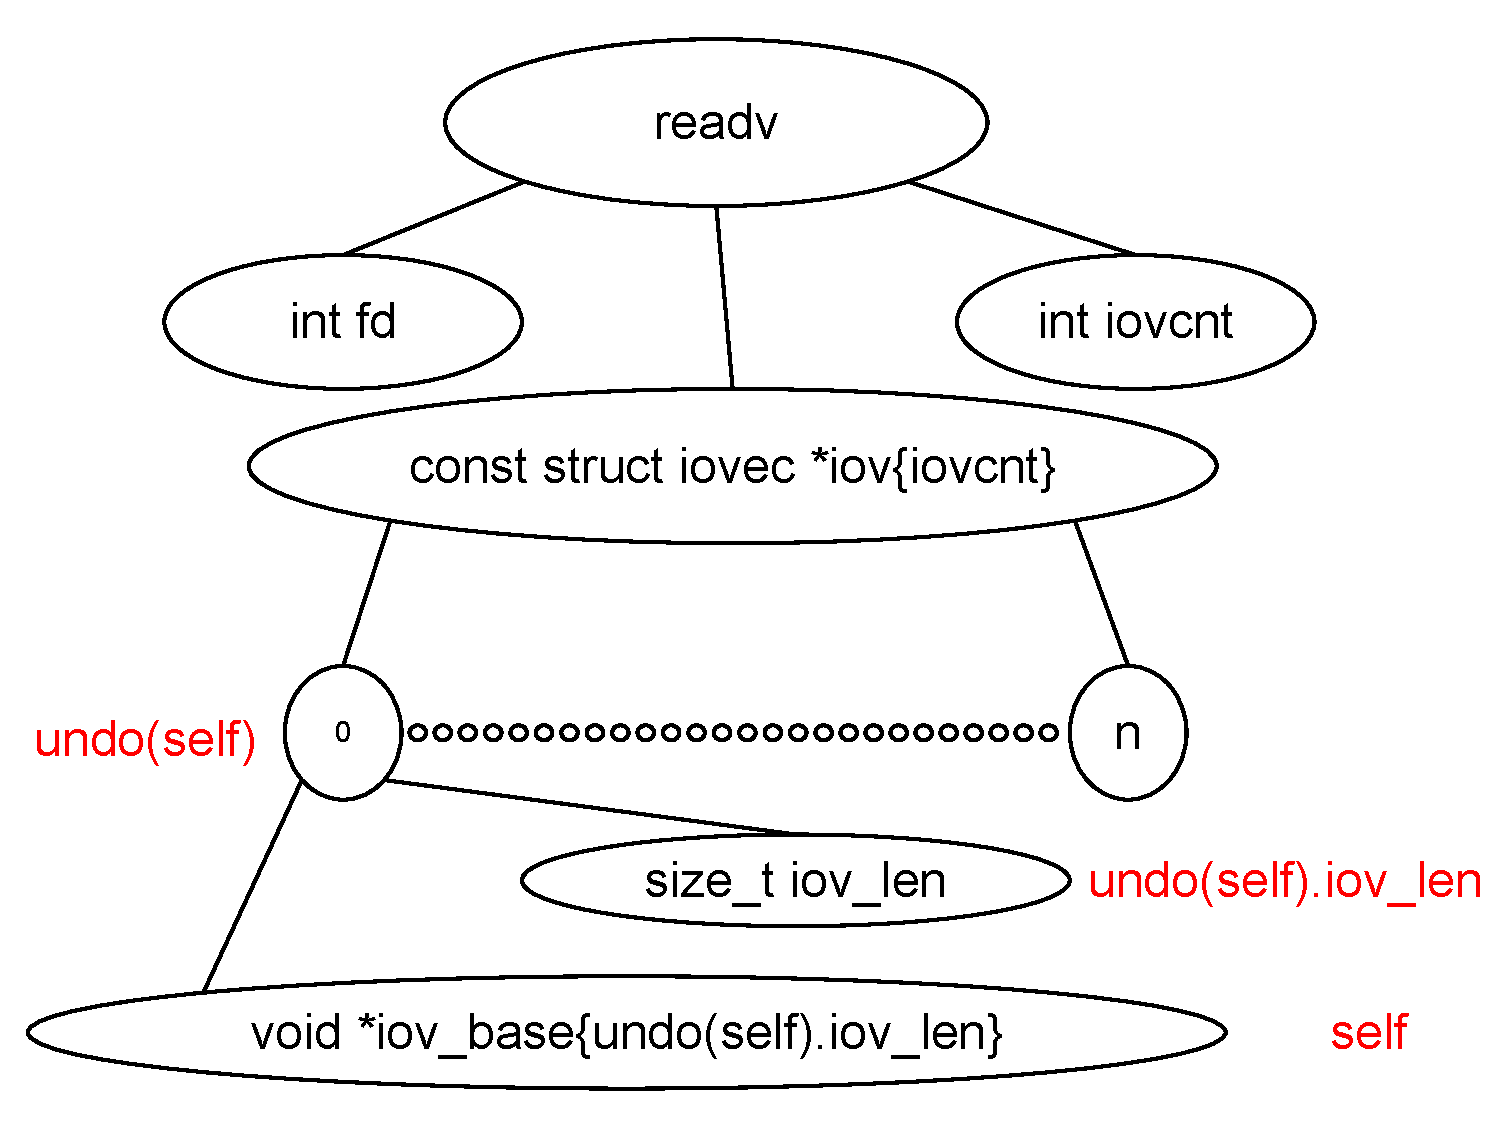
\includegraphics[scale=0.4]{tachyon/LookupDiagram.pdf}
	\end{center}
\caption{A lookup in action}
\label{tach:fig:lookup}
\end{figure}


\tachyon uses lightweight dependent types that can express
relationships between the value of one parameter and the value of
another.  We view types as a tree, and use dependent types to walk the
tree to determine a value.  


The types allow us to walk from the top of the tree, or from the
current parameter.  In \tachyon, we specify {\tt readv} as:
\begin{lstlisting}
ssize_t readv(int fd, const struct inputoutput iovecin *iov{iovcnt}, int iovcnt);
struct iovecin {
  void input *iov_base{undo(self).iov_len};
  size_t iov_len;
}
\end{lstlisting}
We now call the struct \texttt{iovecin}, because while both
\texttt{readv} and \texttt{writev} take an \texttt{iovec}, they are
used differently, and so are assigned differing types (specifically,
in one case the buffers inside are output, while in the other they
are input).  The only new annotations compared to before are
\texttt{undo} and \texttt{self}, which are used to walk the type
tree to reference other fields. The semantic meaning is that
\texttt{iov\_base} is \texttt{iov\_len} bytes.  \texttt{self} refers
to the location at which the current value is being read from.
\texttt{undo} simply says to step back along whatever indexing step
was done to get there.  In this case, this means that \texttt{self}
represents the tree traversal up through that instance of
\texttt{iov\_base}. The ``undo'' brings us up a level, to be looking
at the struct. Then, we index the struct to \texttt{iov\_len} and are
done.  Figure~\ref{tach:fig:lookup} graphically shows the type tree for
\texttt{readv} and how the syntax expresses fields in the tree.

% This is useful as a point of
%reference so that structs can have self contained types, allowing for
%reuse across functions (and can exist in arrays like the one we have
%here).


\subsection{The Tachyon Type System}
The full \tachyon dependent type system is shown in
Figure~\ref{tach:fig:annotations}, and is taken directly from the \tachyon
source code in Haskell.  The language is similar to BNF, where
non-terminals are to the left of the equal sign, and brackets denote
a list (e.g., [A] is a list with elements of type A).


\begin{figure}
\lstset{language=Haskell}
\begin{lstlisting}
data SysSig = SysSig Type [Type]
data Type = Small Int
          | Struct [Type]
          | Ptr IOC Type Bound T
data T = NT | UT
data IOC = In | Out | InOut
data Bound = Const Int | Lookup Lookup
data Lookup = Ret | Arg Int | Index Int Lookup | Self | Undo Lookup
\end{lstlisting}
\caption{The \tachyon annotation language}
\label{tach:fig:annotations}
\end{figure}

In \tachyon's language, IOC represents an IO class, that is, whether
the pointer is input, output, or both.  T represents some form of
termination, to allow us to include null-terminated data. NT is for
null-terminated data; UT is for unterminated data. If a pointer is
null-terminated, reading will cease when a 0 is hit, if this happens prior
to the end of the buffer. The index operation is used on both arrays
and structs, where the $i$'th index refers to the $i$'th field
(counting from 0).

The types available are
\begin{itemize}
\item Small - These correspond to basic integer C types, like
  \texttt{char} or \texttt{long}, and indicate values that should not
  be treated as pointers. The type parameter is the number of bytes of
  the type, e.g., Small(1) is a 1-byte value corresponding to a {\tt
    char}.

\item Struct - an aggregate of other types. Note that previous replay
  work treated such types as raw buffers because they could determine
  size by simply diffing memory before and after a syscall.  In live
  replay, we explicitly lay out all fields because the underlying
  types may yield further information.

\item Ptr - a pointer  annotated with an IO class, the type of
  element it is pointing to, a way to tell how many elements it points
  to, and whether or not it respects a null termination convention.
\end{itemize}

We introduce the concept
of a ``lookup''. This is just a series of steps that can be performed
from either the arguments of a function in the case of an input or
in/out class pointer, or the arguments and return value in the case of
an output pointer, to arrive at a memory location or register. This is
demonstrated in Figure~\ref{tach:fig:lookup}. The Ret and Arg
constructs for a lookup are used to allow us to reference the return
value or various arguments in a system call, respectively.  This is
just the generalization of the tree walking described earlier.

Given this, the encoding of a bound as either a constant or a lookup
is rather natural. It is the use of this bound that makes us lightly
dependently typed---the type depends on the data in question.

Finally, we can build the fundamental structure all this is for---the
system signature.  A system signature, indicated by SysSig, is what is
assigned to each system call in order to allow the tracer to
record and play back its effects. The first parameter is the type of
the return value, and the second is a list of the types of its
arguments.

\paragraph{Type Checking \tachyon Declarations.}

The \tachyon types need only be written once for each system call,
and can be reused for any program.  However, since they are written
manually, we would like to prevent mistakes.  In order to achieve
this, \tachyon also provides type-checking to make sure the
annotations make sense. In particular, \tachyon checks:
\begin{enumerate}
\item Bounds are numbers, not pointers or something else.
\item Bounds use only information which is available for the IO class of the pointer (e.g., input class may not use the return value as a size).
\item Output pointers do not contain structure; they are raw data.
\item Types are potentially compatible with the original C type.
\end{enumerate}
These checks ensure annotations which are usable, self-consistent, and match
the C type. 


%%% Local Variables: 
%%% mode: latex
%%% TeX-master: "paper"
%%% End: 
